\section{Model3DRigid\-Tree  Class Reference}
\label{classModel3DRigidTree}\index{Model3DRigidTree@{Model3DRigid\-Tree}}
A 3D kinematic tree of bodies that uses DH parameters. 


{\tt \#include $<$model3d.h$>$}

Inheritance diagram for Model3DRigid\-Tree::\begin{figure}[H]
\begin{center}
\leavevmode
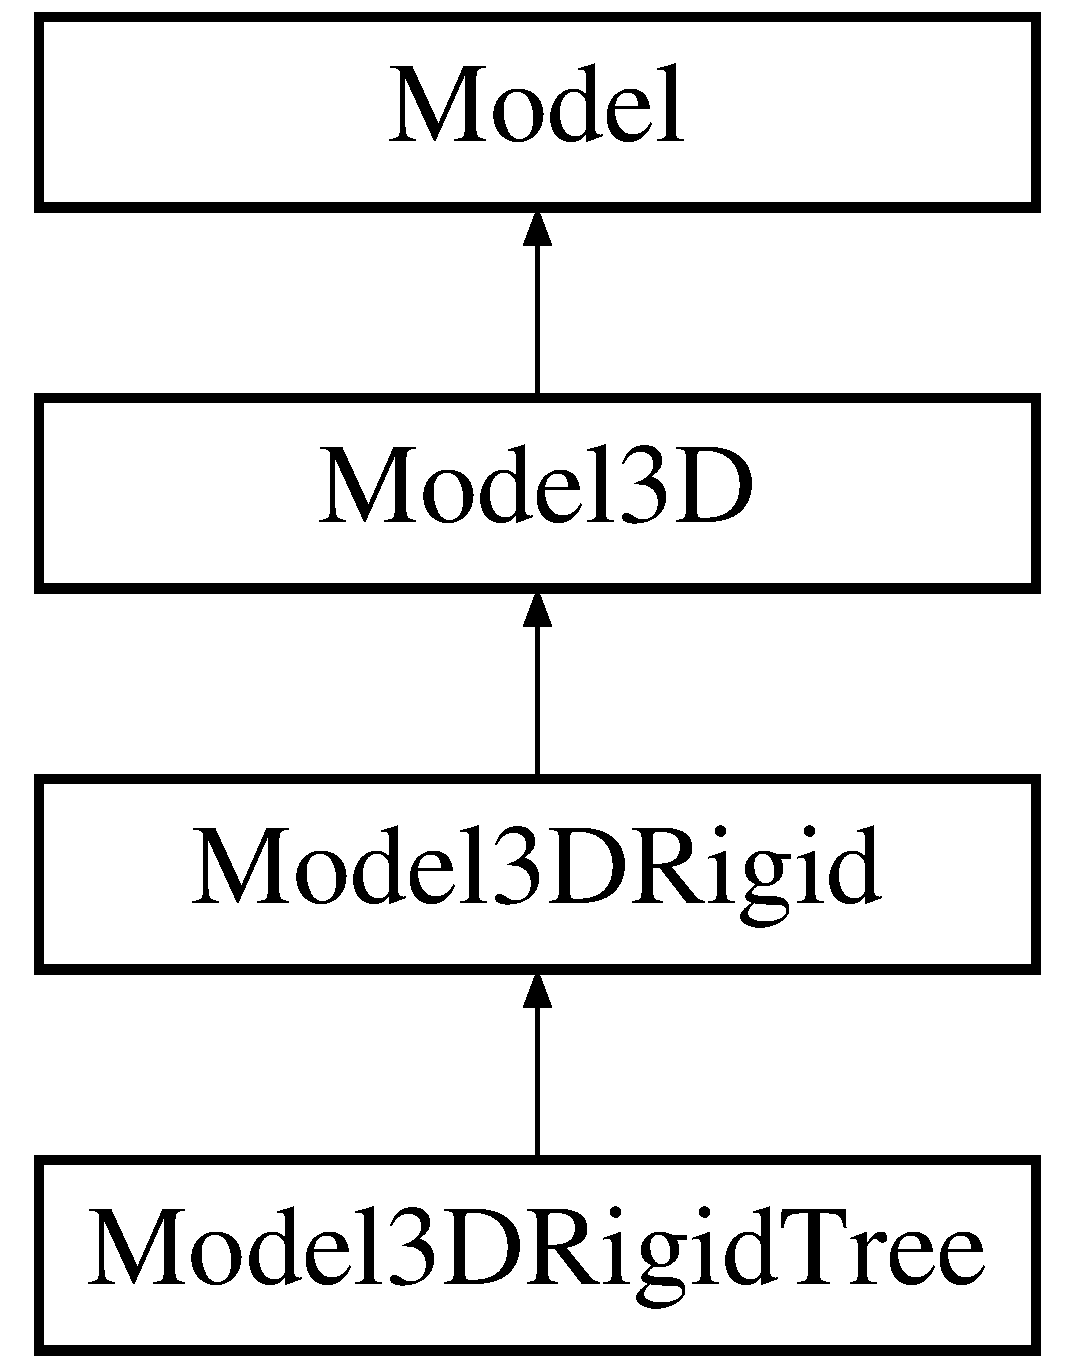
\includegraphics[height=4cm]{classModel3DRigidTree}
\end{center}
\end{figure}
\subsection*{Public Methods}
\begin{CompactItemize}
\item 
{\bf Model3DRigid\-Tree} (string path)
\item 
virtual {\bf $\sim$Model3DRigid\-Tree} ()
\item 
virtual {\bf MSLVector} {\bf State\-Transition\-Equation} (const {\bf MSLVector} \&x, const {\bf MSLVector} \&u)
\begin{CompactList}\small\item\em The state transition equation, or equations of motion, xdot=f(x,u).\item\end{CompactList}\item 
virtual {\bf MSLVector} {\bf State\-To\-Configuration} (const {\bf MSLVector} \&x)
\begin{CompactList}\small\item\em A method that converts a {\bf Model} {\rm (p.\,\pageref{classModel})} state in to a {\bf Geom} {\rm (p.\,\pageref{classGeom})} configuration.\item\end{CompactList}\item 
virtual {\bf MSLVector} {\bf Linear\-Interpolate} (const {\bf MSLVector} \&x1, const {\bf MSLVector} \&x2, const double \&a)
\begin{CompactList}\small\item\em Linearly interpolate two state while respecting topology.\item\end{CompactList}\item 
virtual double {\bf Metric} (const {\bf MSLVector} \&x1, const {\bf MSLVector} \&x2)
\begin{CompactList}\small\item\em A distance metric, which is Euclidean in the base class.\item\end{CompactList}\item 
virtual bool {\bf Satisfied} (const {\bf MSLVector} \&x)
\begin{CompactList}\small\item\em Test whether global state-space constraints are satisfied.\item\end{CompactList}\end{CompactItemize}
\subsection*{Public Attributes}
\begin{CompactItemize}
\item 
int {\bf Num\-Bodies}
\begin{CompactList}\small\item\em Number of bodies in the tree.\item\end{CompactList}\item 
{\bf MSLVector} {\bf DH}
\begin{CompactList}\small\item\em The distances between joints (\char`\"{}a\char`\"{} parameters in kinematics).\item\end{CompactList}\item 
vector$<$int$>$ {\bf State\-Indices}
\item 
vector$<$int$>$ {\bf Parents}
\end{CompactItemize}


\subsection{Detailed Description}
A 3D kinematic tree of bodies that uses DH parameters.

A 3D kinematic tree of bodies that uses DH parameters which should be given in a DH file in the following order: Alpha(1,2...), Theta(1,2...), A(1,2...), D(1,2...). Some of these parameters change during the movement, and each of these parameters becomes a state variable. The indices of these parameters should be given in the file State\-Indices (i.e., each entry corresponds to a state, and indicates which DH parameter is variable). For each body in the tree, the parent body in the tree should be indicated. This is specified in the file Parents. Each entry in Parents corresponds to a body (the i$^\wedge$th element is Robot i). The first entry is the root (this index is ignored because the root has no parent). The bodies in the tree must be arranged so that the indices in Parents are in nondecrreasing order (corresponding, for example to a depth-first search of the tree). 



\subsection{Constructor \& Destructor Documentation}
\index{Model3DRigidTree@{Model3DRigid\-Tree}!Model3DRigidTree@{Model3DRigidTree}}
\index{Model3DRigidTree@{Model3DRigidTree}!Model3DRigidTree@{Model3DRigid\-Tree}}
\subsubsection{\setlength{\rightskip}{0pt plus 5cm}Model3DRigid\-Tree::Model3DRigid\-Tree (string {\em path} = \char`\"{}\char`\"{})}\label{classModel3DRigidTree_a0}


\index{Model3DRigidTree@{Model3DRigid\-Tree}!~Model3DRigidTree@{$\sim$Model3DRigidTree}}
\index{~Model3DRigidTree@{$\sim$Model3DRigidTree}!Model3DRigidTree@{Model3DRigid\-Tree}}
\subsubsection{\setlength{\rightskip}{0pt plus 5cm}Model3DRigid\-Tree::$\sim$Model3DRigid\-Tree ()\hspace{0.3cm}{\tt  [inline, virtual]}}\label{classModel3DRigidTree_a1}




\subsection{Member Function Documentation}
\index{Model3DRigidTree@{Model3DRigid\-Tree}!LinearInterpolate@{LinearInterpolate}}
\index{LinearInterpolate@{LinearInterpolate}!Model3DRigidTree@{Model3DRigid\-Tree}}
\subsubsection{\setlength{\rightskip}{0pt plus 5cm}{\bf MSLVector} Model3DRigid\-Tree::Linear\-Interpolate (const {\bf MSLVector} \& {\em x1}, const {\bf MSLVector} \& {\em x2}, const double \& {\em a})\hspace{0.3cm}{\tt  [virtual]}}\label{classModel3DRigidTree_a4}


Linearly interpolate two state while respecting topology.

If a=0, then x1 is returned; if a=1, then x2 is returned. All intermediate values of \$a $\backslash$in [0,1]\$ yield intermediate states. This method is defined by {\bf Model} {\rm (p.\,\pageref{classModel})}. 

Reimplemented from {\bf Model3DRigid} {\rm (p.\,\pageref{classModel3DRigid_a5})}.\index{Model3DRigidTree@{Model3DRigid\-Tree}!Metric@{Metric}}
\index{Metric@{Metric}!Model3DRigidTree@{Model3DRigid\-Tree}}
\subsubsection{\setlength{\rightskip}{0pt plus 5cm}double Model3DRigid\-Tree::Metric (const {\bf MSLVector} \& {\em x1}, const {\bf MSLVector} \& {\em x2})\hspace{0.3cm}{\tt  [virtual]}}\label{classModel3DRigidTree_a5}


A distance metric, which is Euclidean in the base class.



Reimplemented from {\bf Model3DRigid} {\rm (p.\,\pageref{classModel3DRigid_a4})}.\index{Model3DRigidTree@{Model3DRigid\-Tree}!Satisfied@{Satisfied}}
\index{Satisfied@{Satisfied}!Model3DRigidTree@{Model3DRigid\-Tree}}
\subsubsection{\setlength{\rightskip}{0pt plus 5cm}bool Model3DRigid\-Tree::Satisfied (const {\bf MSLVector} \& {\em x})\hspace{0.3cm}{\tt  [virtual]}}\label{classModel3DRigidTree_a6}


Test whether global state-space constraints are satisfied.



Reimplemented from {\bf Model} {\rm (p.\,\pageref{classModel_a4})}.\index{Model3DRigidTree@{Model3DRigid\-Tree}!StateToConfiguration@{StateToConfiguration}}
\index{StateToConfiguration@{StateToConfiguration}!Model3DRigidTree@{Model3DRigid\-Tree}}
\subsubsection{\setlength{\rightskip}{0pt plus 5cm}{\bf MSLVector} Model3DRigid\-Tree::State\-To\-Configuration (const {\bf MSLVector} \& {\em x})\hspace{0.3cm}{\tt  [virtual]}}\label{classModel3DRigidTree_a3}


A method that converts a {\bf Model} {\rm (p.\,\pageref{classModel})} state in to a {\bf Geom} {\rm (p.\,\pageref{classGeom})} configuration.



Reimplemented from {\bf Model} {\rm (p.\,\pageref{classModel_a8})}.\index{Model3DRigidTree@{Model3DRigid\-Tree}!StateTransitionEquation@{StateTransitionEquation}}
\index{StateTransitionEquation@{StateTransitionEquation}!Model3DRigidTree@{Model3DRigid\-Tree}}
\subsubsection{\setlength{\rightskip}{0pt plus 5cm}{\bf MSLVector} Model3DRigid\-Tree::State\-Transition\-Equation (const {\bf MSLVector} \& {\em x}, const {\bf MSLVector} \& {\em u})\hspace{0.3cm}{\tt  [virtual]}}\label{classModel3DRigidTree_a2}


The state transition equation, or equations of motion, xdot=f(x,u).



Reimplemented from {\bf Model3DRigid} {\rm (p.\,\pageref{classModel3DRigid_a3})}.

\subsection{Member Data Documentation}
\index{Model3DRigidTree@{Model3DRigid\-Tree}!DH@{DH}}
\index{DH@{DH}!Model3DRigidTree@{Model3DRigid\-Tree}}
\subsubsection{\setlength{\rightskip}{0pt plus 5cm}{\bf MSLVector} Model3DRigid\-Tree::DH}\label{classModel3DRigidTree_m1}


The distances between joints (\char`\"{}a\char`\"{} parameters in kinematics).

\index{Model3DRigidTree@{Model3DRigid\-Tree}!NumBodies@{NumBodies}}
\index{NumBodies@{NumBodies}!Model3DRigidTree@{Model3DRigid\-Tree}}
\subsubsection{\setlength{\rightskip}{0pt plus 5cm}int Model3DRigid\-Tree::Num\-Bodies}\label{classModel3DRigidTree_m0}


Number of bodies in the tree.

\index{Model3DRigidTree@{Model3DRigid\-Tree}!Parents@{Parents}}
\index{Parents@{Parents}!Model3DRigidTree@{Model3DRigid\-Tree}}
\subsubsection{\setlength{\rightskip}{0pt plus 5cm}vector$<$ int $>$ Model3DRigid\-Tree::Parents$<$int$>$}\label{classModel3DRigidTree_m3}


\index{Model3DRigidTree@{Model3DRigid\-Tree}!StateIndices@{StateIndices}}
\index{StateIndices@{StateIndices}!Model3DRigidTree@{Model3DRigid\-Tree}}
\subsubsection{\setlength{\rightskip}{0pt plus 5cm}vector$<$ int $>$ Model3DRigid\-Tree::State\-Indices$<$int$>$}\label{classModel3DRigidTree_m2}




The documentation for this class was generated from the following files:\begin{CompactItemize}
\item 
{\bf model3d.h}\item 
{\bf model3d.C}\end{CompactItemize}
